\documentclass[twoside]{book}

% Packages required by doxygen
\usepackage{calc}
\usepackage{doxygen}
\usepackage{graphicx}
\usepackage[utf8]{inputenc}
\usepackage{makeidx}
\usepackage{multicol}
\usepackage{multirow}
\usepackage{textcomp}
\usepackage[table]{xcolor}

% Font selection
\usepackage[T1]{fontenc}
\usepackage{mathptmx}
\usepackage[scaled=.90]{helvet}
\usepackage{courier}
\usepackage{amssymb}
\usepackage{sectsty}
\renewcommand{\familydefault}{\sfdefault}
\allsectionsfont{%
  \fontseries{bc}\selectfont%
  \color{darkgray}%
}
\renewcommand{\DoxyLabelFont}{%
  \fontseries{bc}\selectfont%
  \color{darkgray}%
}

% Page & text layout
\usepackage{geometry}
\geometry{%
  a4paper,%
  top=2.5cm,%
  bottom=2.5cm,%
  left=2.5cm,%
  right=2.5cm%
}
\tolerance=750
\hfuzz=15pt
\hbadness=750
\setlength{\emergencystretch}{15pt}
\setlength{\parindent}{0cm}
\setlength{\parskip}{0.2cm}
\makeatletter
\renewcommand{\paragraph}{%
  \@startsection{paragraph}{4}{0ex}{-1.0ex}{1.0ex}{%
    \normalfont\normalsize\bfseries\SS@parafont%
  }%
}
\renewcommand{\subparagraph}{%
  \@startsection{subparagraph}{5}{0ex}{-1.0ex}{1.0ex}{%
    \normalfont\normalsize\bfseries\SS@subparafont%
  }%
}
\makeatother

% Headers & footers
\usepackage{fancyhdr}
\pagestyle{fancyplain}
\fancyhead[LE]{\fancyplain{}{\bfseries\thepage}}
\fancyhead[CE]{\fancyplain{}{}}
\fancyhead[RE]{\fancyplain{}{\bfseries\leftmark}}
\fancyhead[LO]{\fancyplain{}{\bfseries\rightmark}}
\fancyhead[CO]{\fancyplain{}{}}
\fancyhead[RO]{\fancyplain{}{\bfseries\thepage}}
\fancyfoot[LE]{\fancyplain{}{}}
\fancyfoot[CE]{\fancyplain{}{}}
\fancyfoot[RE]{\fancyplain{}{\bfseries\scriptsize Generated on Thu Apr 3 2014 22\-:16\-:53 for Q\-T Linkbot by Doxygen }}
\fancyfoot[LO]{\fancyplain{}{\bfseries\scriptsize Generated on Thu Apr 3 2014 22\-:16\-:53 for Q\-T Linkbot by Doxygen }}
\fancyfoot[CO]{\fancyplain{}{}}
\fancyfoot[RO]{\fancyplain{}{}}
\renewcommand{\footrulewidth}{0.4pt}
\renewcommand{\chaptermark}[1]{%
  \markboth{#1}{}%
}
\renewcommand{\sectionmark}[1]{%
  \markright{\thesection\ #1}%
}

% Indices & bibliography
\usepackage{natbib}
\usepackage[titles]{tocloft}
\setcounter{tocdepth}{3}
\setcounter{secnumdepth}{5}
\makeindex

% Hyperlinks (required, but should be loaded last)
\usepackage{ifpdf}
\ifpdf
  \usepackage[pdftex,pagebackref=true]{hyperref}
\else
  \usepackage[ps2pdf,pagebackref=true]{hyperref}
\fi
\hypersetup{%
  colorlinks=true,%
  linkcolor=blue,%
  citecolor=blue,%
  unicode%
}

% Custom commands
\newcommand{\clearemptydoublepage}{%
  \newpage{\pagestyle{empty}\cleardoublepage}%
}


%===== C O N T E N T S =====

\begin{document}

% Titlepage & ToC
\hypersetup{pageanchor=false}
\pagenumbering{roman}
\begin{titlepage}
\vspace*{7cm}
\begin{center}%
{\Large Q\-T Linkbot }\\
\vspace*{1cm}
{\large Generated by Doxygen 1.8.6}\\
\vspace*{0.5cm}
{\small Thu Apr 3 2014 22:16:53}\\
\end{center}
\end{titlepage}
\clearemptydoublepage
\tableofcontents
\clearemptydoublepage
\pagenumbering{arabic}
\hypersetup{pageanchor=true}

%--- Begin generated contents ---
\chapter{Hierarchical Index}
\section{Class Hierarchy}
This inheritance list is sorted roughly, but not completely, alphabetically\-:\begin{DoxyCompactList}
\item C\-Linkbot\begin{DoxyCompactList}
\item \contentsline{section}{Q\-Linkbot}{\pageref{class_q_linkbot}}{}
\end{DoxyCompactList}
\item Q\-Object\begin{DoxyCompactList}
\item \contentsline{section}{Q\-Linkbot}{\pageref{class_q_linkbot}}{}
\item \contentsline{section}{Q\-Linkbot\-Worker}{\pageref{class_q_linkbot_worker}}{}
\end{DoxyCompactList}
\end{DoxyCompactList}

\chapter{Class Index}
\section{Class List}
Here are the classes, structs, unions and interfaces with brief descriptions\-:\begin{DoxyCompactList}
\item\contentsline{section}{\hyperlink{class_q_linkbot}{Q\-Linkbot} }{\pageref{class_q_linkbot}}{}
\item\contentsline{section}{\hyperlink{class_q_linkbot_worker}{Q\-Linkbot\-Worker} }{\pageref{class_q_linkbot_worker}}{}
\end{DoxyCompactList}

\chapter{Class Documentation}
\hypertarget{class_q_linkbot}{\section{Q\-Linkbot Class Reference}
\label{class_q_linkbot}\index{Q\-Linkbot@{Q\-Linkbot}}
}
Inheritance diagram for Q\-Linkbot\-:\begin{figure}[H]
\begin{center}
\leavevmode
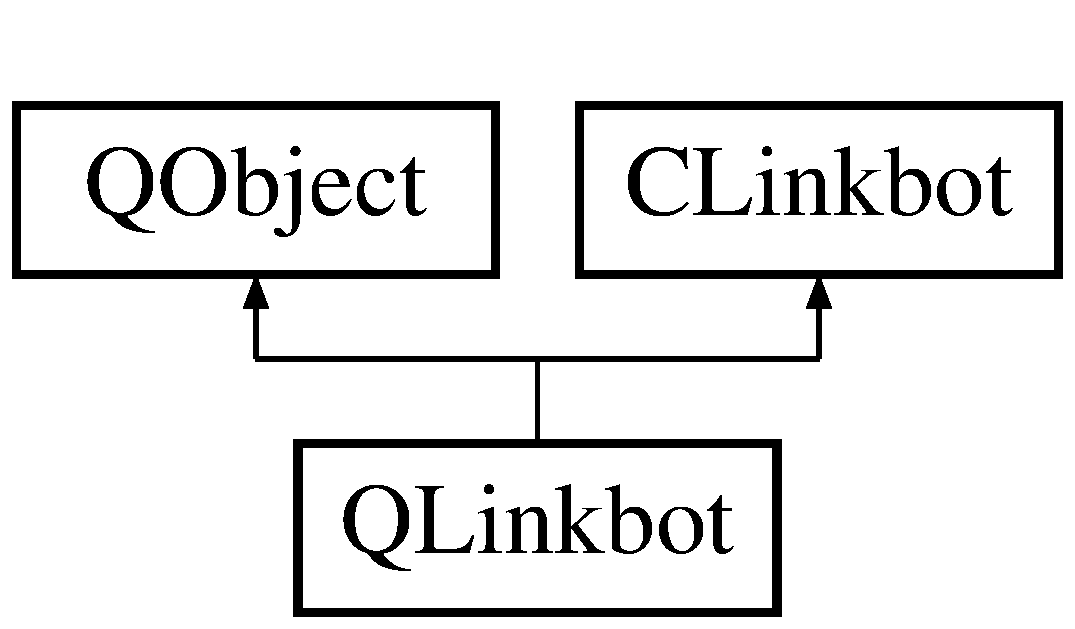
\includegraphics[height=2.000000cm]{class_q_linkbot}
\end{center}
\end{figure}
\subsection*{Public Slots}
\begin{DoxyCompactItemize}
\item 
\hypertarget{class_q_linkbot_a005462b48ca50175a9f27e7ea58c9acb}{void {\bfseries new\-Accel\-Values} (double x, double y, double z)}\label{class_q_linkbot_a005462b48ca50175a9f27e7ea58c9acb}

\item 
\hypertarget{class_q_linkbot_af6ccf5b180ecd88d43dad868d0f28e38}{void {\bfseries new\-Button\-Values} (int button, int button\-Down)}\label{class_q_linkbot_af6ccf5b180ecd88d43dad868d0f28e38}

\item 
\hypertarget{class_q_linkbot_a62cf029f23de74872433b69e42b5d094}{void {\bfseries new\-Motor\-Values} (double j1, double j2, double j3, int mask)}\label{class_q_linkbot_a62cf029f23de74872433b69e42b5d094}

\end{DoxyCompactItemize}
\subsection*{Signals}
\begin{DoxyCompactItemize}
\item 
\hypertarget{class_q_linkbot_afff0d6647281757fa2a064d9e25b26d6}{void {\bfseries button\-Changed} (\hyperlink{class_q_linkbot}{Q\-Linkbot} $\ast$linkbot, int button, int event)}\label{class_q_linkbot_afff0d6647281757fa2a064d9e25b26d6}

\item 
\hypertarget{class_q_linkbot_ac5601889a86f48fc609dfb98cbd8a15e}{void {\bfseries joints\-Changed} (\hyperlink{class_q_linkbot}{Q\-Linkbot} $\ast$linkbot, double j1, double j2, double j3, int mask)}\label{class_q_linkbot_ac5601889a86f48fc609dfb98cbd8a15e}

\item 
\hypertarget{class_q_linkbot_abd078d585f5b7c251aac051f4d74d5f2}{void {\bfseries joint\-Changed} (\hyperlink{class_q_linkbot}{Q\-Linkbot} $\ast$linkbot, int joint, double angle\-Position)}\label{class_q_linkbot_abd078d585f5b7c251aac051f4d74d5f2}

\item 
\hypertarget{class_q_linkbot_ac35fe57149cabea92c491db247a722e9}{void {\bfseries accel\-Changed} (\hyperlink{class_q_linkbot}{Q\-Linkbot} $\ast$linkbot, double x, double y, double z)}\label{class_q_linkbot_ac35fe57149cabea92c491db247a722e9}

\end{DoxyCompactItemize}
\subsection*{Public Member Functions}
\begin{DoxyCompactItemize}
\item 
\hypertarget{class_q_linkbot_aa1f41b061c82c1cb581d7a8be8cbef9e}{virtual void {\bfseries connect\-Robot} (const Q\-String \&id)}\label{class_q_linkbot_aa1f41b061c82c1cb581d7a8be8cbef9e}

\item 
\hypertarget{class_q_linkbot_ab6903f8b9f8d0f78bef4690dd2f30038}{virtual void {\bfseries disconnect\-Robot} ()}\label{class_q_linkbot_ab6903f8b9f8d0f78bef4690dd2f30038}

\item 
\hypertarget{class_q_linkbot_a7e156b431df408db2a7a5e931a64c70b}{virtual int {\bfseries enable\-Accel\-Event\-Callback} ()}\label{class_q_linkbot_a7e156b431df408db2a7a5e931a64c70b}

\item 
\hypertarget{class_q_linkbot_affd651759494b44d6c2b63c38eaa7dd2}{virtual int {\bfseries enable\-Button\-Callback} ()}\label{class_q_linkbot_affd651759494b44d6c2b63c38eaa7dd2}

\item 
\hypertarget{class_q_linkbot_a44190b9f975f35480ac484724a6f70d4}{virtual int {\bfseries enable\-Joint\-Event\-Callback} ()}\label{class_q_linkbot_a44190b9f975f35480ac484724a6f70d4}

\item 
\hypertarget{class_q_linkbot_a40a942fe57ef1a244f4fbf5b6a8ae8ff}{virtual Q\-String {\bfseries get\-Serial\-I\-D} () const }\label{class_q_linkbot_a40a942fe57ef1a244f4fbf5b6a8ae8ff}

\item 
\hypertarget{class_q_linkbot_a148e1892efa406a64467ac53292ae901}{void {\bfseries lock} ()}\label{class_q_linkbot_a148e1892efa406a64467ac53292ae901}

\item 
\hypertarget{class_q_linkbot_a13af1ef77a0a2c83c6ea090fcb2f3988}{void {\bfseries unlock} ()}\label{class_q_linkbot_a13af1ef77a0a2c83c6ea090fcb2f3988}

\item 
\hypertarget{class_q_linkbot_a9cbfa651dcb09f00eb8417fc3c885784}{bool {\bfseries operator==} (const \hyperlink{class_q_linkbot}{Q\-Linkbot} \&other)}\label{class_q_linkbot_a9cbfa651dcb09f00eb8417fc3c885784}

\item 
\hypertarget{class_q_linkbot_a799bbadfc9f1c0f34d110c60bb935590}{bool {\bfseries operator!=} (const \hyperlink{class_q_linkbot}{Q\-Linkbot} \&other)}\label{class_q_linkbot_a799bbadfc9f1c0f34d110c60bb935590}

\end{DoxyCompactItemize}


The documentation for this class was generated from the following files\-:\begin{DoxyCompactItemize}
\item 
E\-:/\-Users/\-Adam/\-Documents/\-Git\-Hub/qlinkbot/include/Q\-Linkbot.\-h\item 
E\-:/\-Users/\-Adam/\-Documents/\-Git\-Hub/qlinkbot/src/Q\-Linkbot.\-cpp\end{DoxyCompactItemize}

\hypertarget{class_q_linkbot_worker}{\section{Q\-Linkbot\-Worker Class Reference}
\label{class_q_linkbot_worker}\index{Q\-Linkbot\-Worker@{Q\-Linkbot\-Worker}}
}
Inheritance diagram for Q\-Linkbot\-Worker\-:\begin{figure}[H]
\begin{center}
\leavevmode
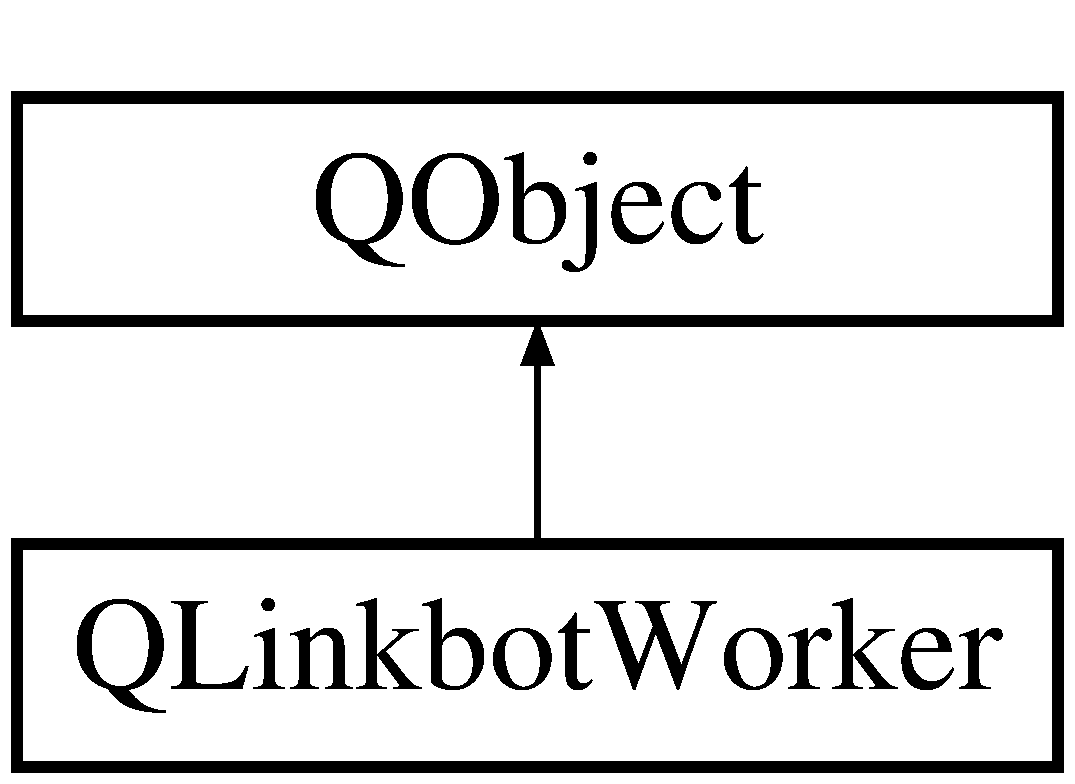
\includegraphics[height=2.000000cm]{class_q_linkbot_worker}
\end{center}
\end{figure}
\subsection*{Public Slots}
\begin{DoxyCompactItemize}
\item 
\hypertarget{class_q_linkbot_worker_a36ad2672be55711016508b62237449fc}{void {\bfseries do\-Work} ()}\label{class_q_linkbot_worker_a36ad2672be55711016508b62237449fc}

\end{DoxyCompactItemize}
\subsection*{Signals}
\begin{DoxyCompactItemize}
\item 
\hypertarget{class_q_linkbot_worker_a7e7b07ddc566a45d3b4be92bae37cfc4}{void {\bfseries accel\-Changed} (double x, double y, double z)}\label{class_q_linkbot_worker_a7e7b07ddc566a45d3b4be92bae37cfc4}

\item 
\hypertarget{class_q_linkbot_worker_a9233a3905a96f73484d0fa269e59f2c3}{void {\bfseries button\-Changed} (int button, int button\-Down)}\label{class_q_linkbot_worker_a9233a3905a96f73484d0fa269e59f2c3}

\item 
\hypertarget{class_q_linkbot_worker_a2c7f4271721afe32fef9a91cf2b44b94}{void {\bfseries motor\-Changed} (double j1, double j2, double j3, int mask)}\label{class_q_linkbot_worker_a2c7f4271721afe32fef9a91cf2b44b94}

\end{DoxyCompactItemize}
\subsection*{Public Member Functions}
\begin{DoxyCompactItemize}
\item 
\hypertarget{class_q_linkbot_worker_add984ed6b839959ac0e58928f1511abf}{{\bfseries Q\-Linkbot\-Worker} (\hyperlink{class_q_linkbot}{Q\-Linkbot} $\ast$linkbot)}\label{class_q_linkbot_worker_add984ed6b839959ac0e58928f1511abf}

\item 
\hypertarget{class_q_linkbot_worker_ad4d5aa10b15dbac7118a466e8245bf29}{void {\bfseries set\-New\-Accel\-Values} (double x, double y, double z)}\label{class_q_linkbot_worker_ad4d5aa10b15dbac7118a466e8245bf29}

\item 
\hypertarget{class_q_linkbot_worker_ab19d62d665270906afee0e198c2b2541}{void {\bfseries set\-New\-Button\-Values} (int button, int down)}\label{class_q_linkbot_worker_ab19d62d665270906afee0e198c2b2541}

\item 
\hypertarget{class_q_linkbot_worker_af5dc38b873ce3aedfd96f10e098b2053}{void {\bfseries set\-New\-Motor\-Values} (double j1, double j2, double j3, int mask)}\label{class_q_linkbot_worker_af5dc38b873ce3aedfd96f10e098b2053}

\end{DoxyCompactItemize}


The documentation for this class was generated from the following files\-:\begin{DoxyCompactItemize}
\item 
E\-:/\-Users/\-Adam/\-Documents/\-Git\-Hub/qlinkbot/include/Q\-Linkbot.\-h\item 
E\-:/\-Users/\-Adam/\-Documents/\-Git\-Hub/qlinkbot/src/Q\-Linkbot.\-cpp\end{DoxyCompactItemize}

%--- End generated contents ---

% Index
\newpage
\phantomsection
\addcontentsline{toc}{chapter}{Index}
\printindex

\end{document}
